\documentclass{standalone}

\usepackage{tikz,pgf} %and any other packages or tikzlibraries your picture needs

\begin{document}

\begin{center}
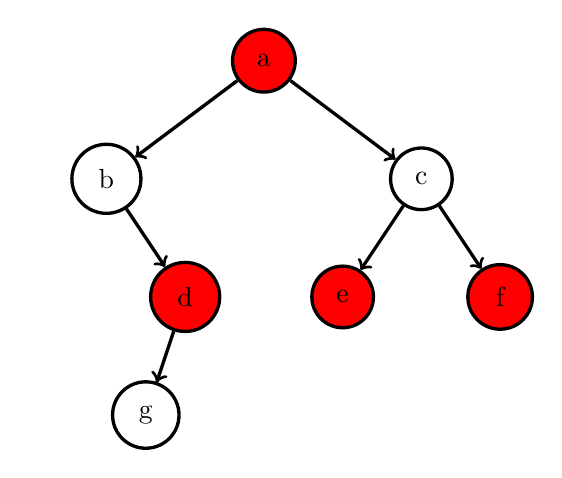
\begin{tikzpicture}[
  level distance=6mm,
  every node/.style={text ragged, inner sep=2mm}
]
\tikzstyle{level 1}=[sibling distance=4cm,level distance=1.5cm]
\tikzstyle{level 2}=[sibling distance=2cm, level distance=1.5cm]
\tikzstyle{level 3}=[sibling distance=1cm, level distance=1.5cm]
\tikzstyle{kant}=[circle, text width=1cm, text centered, sloped]
\tikzstyle{punkt}=[circle, draw=black, very thick]

\path[punkt, ->]
  node [punkt, fill=red, text=black] {a}
  child {
    node [punkt, text=black] {b}
    child [fill=none] {edge from parent[draw=none]}
    child {
      node [punkt, fill=red, text=black] {d}
      child {
        node [punkt, text=black] {g}
        [fill=none] {edge from parent[draw=none]}
        [fill=none] {edge from parent[draw=none]}
      }
      child [fill=none] {edge from parent[draw=none]}
    }
  }
  child {
    node [punkt, text=black] {c}
    child {
      node[punkt, fill=red, text=black] {e}
    }
    child {
      node[punkt, fill=red,  text=black] {f}
    }
  };
\end{tikzpicture}
\end{center}

\end{document}
